\begin{figure}[htbp]
	\centering
	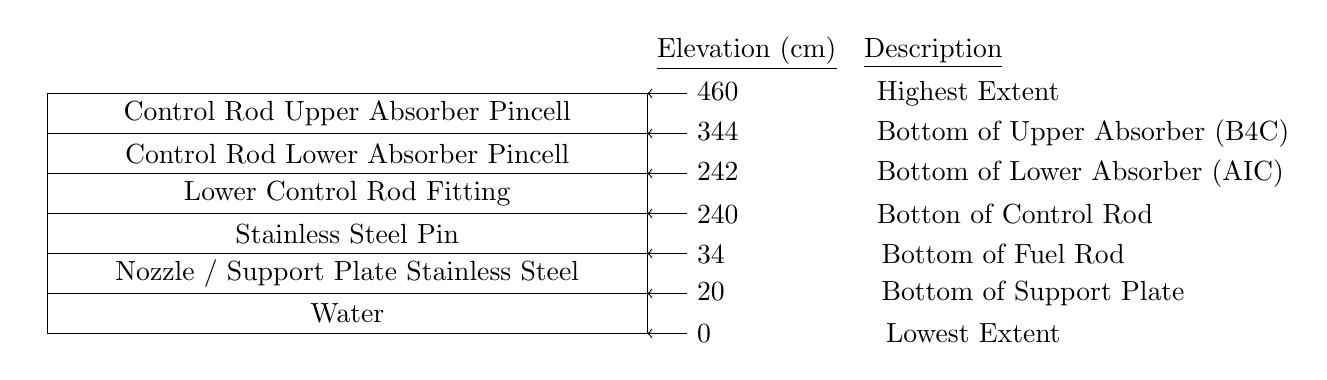
\begin{tikzpicture}[scale=1,x=1in,y=1in]
	\node[inner sep=0pt,
	text width=3 in,
	minimum size=0.2 in,
	draw=black,
	align=center,
	shift={(0,0.0)}] (n0) {Water};
	\draw[->] (1.7,-0.1) node[right,anchor=west] {0 ~~~~~~~~~~~~~~~~~ Lowest Extent} -- (1.5,-0.1);
	\node[anchor=east] (s0) at (n0.west) {};
	\node[inner sep=0pt,
	text width=3 in,
	minimum size=0.2 in,
	draw=black,
	align=center,
	shift={(0,0.2)}] (n1) {Nozzle / Support Plate Stainless Steel};
	\draw[->] (1.7,0.1) node[right,anchor=west] {20 ~~~~~~~~~~~~~~~ Bottom of Support Plate} -- (1.5,0.1);
	\node[inner sep=0pt,
	text width=3 in,
	minimum size=0.2 in,
	draw=black,
	align=center,
	shift={(0,0.4)}] (n2) {Stainless Steel Pin};
	\draw[->] (1.7,0.3) node[right,anchor=west] {34 ~~~~~~~~~~~~~~~ Bottom of Fuel Rod} -- (1.5,0.3);
	\node[inner sep=0pt,
	text width=3 in,
	minimum size=0.2 in,
	draw=black,
	align=center,
	shift={(0,0.6)}] (n3) {Lower Control Rod Fitting};
	\draw[->] (1.7,0.5) node[right,anchor=west] {240 ~~~~~~~~~~~~~ Botton of Control Rod} -- (1.5,0.5);
	
	\node[inner sep=0pt,
	text width=3 in,
	minimum size=0.2 in,
	draw=black,
	align=center,
	shift={(0,0.8)}] (n4) {Control Rod Lower Absorber Pincell};
	\draw[->] (1.7,0.7) node[right,anchor=west] {242 ~~~~~~~~~~~~~ Bottom of Lower Absorber (AIC)} -- (1.5,0.7);
	\node[inner sep=0pt,
	text width=3 in,
	minimum size=0.2 in,
	draw=black,
	align=center,
	shift={(0,1.0)}] (n5) {Control Rod Upper Absorber Pincell};
	\draw[->] (1.7,0.9) node[right,anchor=west] {344 ~~~~~~~~~~~~~ Bottom of Upper Absorber (B4C)} -- (1.5,0.9);
	
	\draw[->] (1.7,1.1) node[right,anchor=west] {460 ~~~~~~~~~~~~~ Highest Extent} -- (1.5,1.1);
	\draw (1.5,1.3) node[right,anchor=west] {\underline{Elevation (cm)} ~ \underline{Description}};
	
	\end{tikzpicture}
	
	
	\caption[Control Rod Insertion]{Control rod pincell axial specification for the single assembly control rod insertion model.\label{fig:control-rod-spec}}
\end{figure}
